% Options for packages loaded elsewhere
\PassOptionsToPackage{unicode}{hyperref}
\PassOptionsToPackage{hyphens}{url}
%
\documentclass[
  12pt,
]{article}
\title{WEB-BASED TOOLS FOR DATA ANALYSIS: JUPYTERLAB ENVIRONMENT AND
WORKFLOW OPTIMIZATION}
\author{Miguel Portela}
\date{October 2021}

\usepackage{amsmath,amssymb}
\usepackage{lmodern}
\usepackage{iftex}
\ifPDFTeX
  \usepackage[T1]{fontenc}
  \usepackage[utf8]{inputenc}
  \usepackage{textcomp} % provide euro and other symbols
\else % if luatex or xetex
  \usepackage{unicode-math}
  \defaultfontfeatures{Scale=MatchLowercase}
  \defaultfontfeatures[\rmfamily]{Ligatures=TeX,Scale=1}
  \setmainfont[]{Times New Roman}
  \setsansfont[]{Times New Roman}
\fi
% Use upquote if available, for straight quotes in verbatim environments
\IfFileExists{upquote.sty}{\usepackage{upquote}}{}
\IfFileExists{microtype.sty}{% use microtype if available
  \usepackage[]{microtype}
  \UseMicrotypeSet[protrusion]{basicmath} % disable protrusion for tt fonts
}{}
\makeatletter
\@ifundefined{KOMAClassName}{% if non-KOMA class
  \IfFileExists{parskip.sty}{%
    \usepackage{parskip}
  }{% else
    \setlength{\parindent}{0pt}
    \setlength{\parskip}{6pt plus 2pt minus 1pt}}
}{% if KOMA class
  \KOMAoptions{parskip=half}}
\makeatother
\usepackage{xcolor}
\IfFileExists{xurl.sty}{\usepackage{xurl}}{} % add URL line breaks if available
\IfFileExists{bookmark.sty}{\usepackage{bookmark}}{\usepackage{hyperref}}
\hypersetup{
  pdftitle={WEB-BASED TOOLS FOR DATA ANALYSIS: JUPYTERLAB ENVIRONMENT AND WORKFLOW OPTIMIZATION},
  pdfauthor={Miguel Portela},
  hidelinks,
  pdfcreator={LaTeX via pandoc}}
\urlstyle{same} % disable monospaced font for URLs
\usepackage[paperwidth=210mm,paperheight=297mm,left=27mm,right=27mm,top=27mm,bottom=27mm]{geometry}
\usepackage{graphicx}
\makeatletter
\def\maxwidth{\ifdim\Gin@nat@width>\linewidth\linewidth\else\Gin@nat@width\fi}
\def\maxheight{\ifdim\Gin@nat@height>\textheight\textheight\else\Gin@nat@height\fi}
\makeatother
% Scale images if necessary, so that they will not overflow the page
% margins by default, and it is still possible to overwrite the defaults
% using explicit options in \includegraphics[width, height, ...]{}
\setkeys{Gin}{width=\maxwidth,height=\maxheight,keepaspectratio}
% Set default figure placement to htbp
\makeatletter
\def\fps@figure{htbp}
\makeatother
\setlength{\emergencystretch}{3em} % prevent overfull lines
\providecommand{\tightlist}{%
  \setlength{\itemsep}{0pt}\setlength{\parskip}{0pt}}
\setcounter{secnumdepth}{-\maxdimen} % remove section numbering
\usepackage{pdfpages}
\usepackage{graphicx}
\ifLuaTeX
  \usepackage{selnolig}  % disable illegal ligatures
\fi

\begin{document}
\maketitle

\hypertarget{web-based-tools-for-data-analysis-jupyterlab-environment-and-workflow-optimization}{%
\subsection{WEB-BASED TOOLS FOR DATA ANALYSIS: JUPYTERLAB ENVIRONMENT
AND WORKFLOW
OPTIMIZATION}\label{web-based-tools-for-data-analysis-jupyterlab-environment-and-workflow-optimization}}

\hypertarget{miguel-portela}{%
\subsubsection{Miguel Portela}\label{miguel-portela}}

\begin{quote}
October 2021
\end{quote}

\textbf{The following material is available on GitHub}

\url{https://github.com/reisportela/R_Training}

\href{https://mybinder.org/v2/gh/reisportela/R_Training/HEAD?urlpath=lab}{\includegraphics{https://mybinder.org/badge_logo.svg}}

\hypertarget{operating-system}{%
\section{1. Operating system}\label{operating-system}}

\begin{itemize}
\tightlist
\item
  Linux (e.g., Ubuntu 20.04), OSX Catalina, Windows 10
\end{itemize}

\hypertarget{packages}{%
\section{2. Packages}\label{packages}}

\begin{quote}
\textbf{Windows}: consider installing
\href{https://chocolatey.org/}{Chocolatey}, a package manager for
Windows (similar to \texttt{yum} in CentOS or \texttt{brew} in OSX)
\end{quote}

\begin{itemize}
\tightlist
\item
  Python: install Anaconda --
  \href{https://www.anaconda.com/}{https://www.anaconda.com}
\end{itemize}

\begin{quote}
\textbf{Example, using Chocolatey}: \texttt{choco\ install\ anaconda3}

or download and install
\end{quote}

\begin{itemize}
\tightlist
\item
  \textbf{R}:
  \href{https://www.r-project.org/}{https://www.r-project.org}
\item
  \textbf{Julia}: \href{https://julialang.org/}{https://julialang.org}
\item
  \textbf{Stata}: \href{https://www.stata.com/}{https://www.stata.com}
\end{itemize}

\begin{quote}
Recomendation: install
\href{https://rstudio.com/products/rstudio/download/}{RStudio}
\end{quote}

\hypertarget{jupyter}{%
\section{\texorpdfstring{3.
\href{https://jupyter.org/}{Jupyter}}{3. Jupyter}}\label{jupyter}}

\begin{quote}
``The Jupyter Notebook is an open-source web application that allows you
to \textbf{create and share} documents that contain \emph{live code},
equations, visualizations and \textbf{narrative text}. Uses include:
data cleaning and transformation, numerical simulation, statistical
modeling, data visualization, machine learning, and much more.''
\end{quote}

\hypertarget{install-jupyter}{%
\subsection{\texorpdfstring{3.1 Install
\href{https://jupyter.org/install}{jupyter}}{3.1 Install jupyter}}\label{install-jupyter}}

\begin{itemize}
\tightlist
\item
  Open a Terminal in either Linux or OSX
\item
  Open Windows Powershell as Administrator
\end{itemize}

\emph{\emph{Run the following lines}}

\begin{itemize}
\tightlist
\item
  \textbf{jupyter notebook}: \emph{pip install notebook} \textbf{or}
  \emph{conda install -c conda-forge notebook}
\item
  \textbf{jupyter lab}: \emph{pip install jupyterlab} \textbf{or}
  \emph{conda install -c conda-forge jupyterlab}
\end{itemize}

\hypertarget{install-your-kernels}{%
\subsection{\texorpdfstring{3.2 Install your
\href{https://github.com/jupyter/jupyter/wiki/Jupyter-kernels}{kernels}}{3.2 Install your kernels}}\label{install-your-kernels}}

\begin{itemize}
\item
  \textbf{Python}: this should be the first one installed
  \href{https://pypi.org/project/ipykernel/}{ipykernel}
\item
  \textbf{R}: \href{https://irkernel.github.io/installation/}{irkernel}

  Open an R console, e.g.~within RStudio, and execute sequentially,
  \emph{install.packages(`IRkernel')}, \emph{IRkernel::installspec()}

  Add \texttt{Node.js} and \texttt{npm}

  Visit \href{https://nodejs.org/en/download/}{Nodejs.org} to
  \textbf{install} \texttt{Node.js} and \texttt{npm}
\item
  \textbf{Julia}: \href{https://github.com/JuliaLang/IJulia.jl}{IJulia}

  Run Julia and execute sequentially, \emph{using Pkg},
  \emph{Pkg.add(``IJulia'')}
\item
  \textbf{Stata}:
  \href{https://github.com/kylebarron/stata_kernel}{stata\_kernel}
\end{itemize}

\begin{quote}
for Stata see the instructions by
\href{https://kylebarron.dev/stata_kernel/getting_started/}{Kyle Barron}

\href{https://kylebarron.dev/stata_kernel/using_stata_kernel/magics/}{Magics}
-- ``Magics are programs provided by stata\_kernel that enhance the
experience of working with Stata in Jupyter.''
\end{quote}

\hypertarget{start-notebook-or-lab}{%
\subsection{3.3 Start `notebook' or `lab'}\label{start-notebook-or-lab}}

Open a \texttt{Terminal}/\texttt{Power\ shell}, move to your working
folder and type:

\begin{itemize}
\item
  \textbf{jupyter notebook}: \emph{jupyter notebook}
\item
  \textbf{jupyter lab}: \emph{jupyter lab}
\end{itemize}

It should open your browser with the notebook and the installed kernels.

\hypertarget{remove-a-kernel}{%
\subsection{3.4 Remove a Kernel}\label{remove-a-kernel}}

\begin{quote}
\texttt{jupyter\ kernelspec\ list}

\texttt{jupyter\ kernelspec\ uninstall\ unwanted-kernel}
\end{quote}

\hypertarget{binder}{%
\section{\texorpdfstring{4.
\href{https://jupyter.org/binder}{Binder}}{4. Binder}}\label{binder}}

\href{https://www.r-bloggers.com/running-r-projects-in-mybinder-dockerfile-creation-with-holepunch/}{Running
R Projects in MyBinder: Dockerfile Creation With Holepunch}

\begin{itemize}
\tightlist
\item
  myBinder
\item
  Gesis Notebooks
\end{itemize}

Check the following link

\href{https://mybinder.readthedocs.io/en/latest/using/config_files.html}{Configuration
Files}

\textbf{mybinder} allows you to create a linked icon to your interactive
notebook

\begin{quote}
\href{https://mybinder.org/v2/gh/reisportela/R_Training/HEAD?urlpath=lab}{\includegraphics{https://mybinder.org/badge_logo.svg}}
\end{quote}

\begin{quote}
Check the example in GitHub with RStudio \& R 3.6 + Python + Julia +
Stata
\end{quote}

\href{https://github.com/reisportela/prjs}{\texttt{reisportela/prjs}}

\begin{itemize}
\tightlist
\item
  or a setup where we can build a notebook with Python 3.0 or R (you can
  also run RStudio from this link)
\end{itemize}

\href{https://mybinder.org/v2/gh/reisportela/prjs/master}{\includegraphics{https://mybinder.org/badge_logo.svg}}

Even better, use \href{https://notebooks.gesis.org/hub/home}{GESIS
notebooks} to launch your image

\href{https://notebooks.gesis.org/user/reisportela@gmail.com}{The
concept using GESIS}

MyBinder: \href{https://github.com/binder-examples}{EXAMPLES}

\hypertarget{a-gallery-of-interesting-jupyter-notebooks}{%
\section{5. A gallery of interesting Jupyter
Notebooks}\label{a-gallery-of-interesting-jupyter-notebooks}}

\begin{itemize}
\item
  \href{https://github.com/jupyter/jupyter/wiki/A-gallery-of-interesting-Jupyter-Notebooks}{Gallery}
\item
  \href{https://swcarpentry.github.io/python-novice-gapminder/}{Plotting
  and Programming in Python}
\item
  \href{https://nbviewer.jupyter.org/github/Tanu-N-Prabhu/Python/blob/master/Exploratory_data_Analysis.ipynb}{Exploratory
  data analysis in Python}
\end{itemize}

\hypertarget{books}{%
\section{6. Books}\label{books}}

\begin{itemize}
\item
  \href{https://jakevdp.github.io/PythonDataScienceHandbook/}{Python
  Data Science Handbook}
\item
  \href{https://bookdown.org/}{Bookdown}
\item
  \href{https://www.youtube.com/watch?v=rJsWJMBksK0}{How to Hide all the
  code cells in Jupyter Notebook Python with single Click}
\end{itemize}

\hypertarget{checks}{%
\section{7. Checks}\label{checks}}

\begin{itemize}
\item
  \href{https://github.com/binder-examples/multi-language-demo}{Binder
  Multi-language demo}
\item
  \href{https://mybinder.readthedocs.io/en/latest/index.html}{mybinder.io}
\end{itemize}

\hypertarget{sos-notebook}{%
\section{\texorpdfstring{8. SoS
\href{https://vatlab.github.io/sos-docs/}{NOTEBOOK}}{8. SoS NOTEBOOK}}\label{sos-notebook}}

\begin{itemize}
\tightlist
\item
  \href{https://vatlab.github.io/sos-docs/running.html\#Local-installation}{Local
  installation}
\end{itemize}

\hypertarget{pip-installation}{%
\subsection{pip installation}\label{pip-installation}}

pip3 install sos

pip3 install sos-pbs

pip3 install sos-notebook

pip3 install sos-papermill

pip3 install sos-r

pip3 install sos-julia

pip3 install sos-stata

python3 -m sos\_notebook.install

jupyter kernelspec list

jupyter notebook

\hypertarget{discussion-on-julia}{%
\section{9. Discussion on Julia}\label{discussion-on-julia}}

\begin{itemize}
\item
  use an environment
  \href{https://github.com/binder-examples/julia-python}{julia-python}
\item
  a
  \href{https://blog.jupyter.org/i-python-you-r-we-julia-baf064ca1fb6}{multi-language-demo}
\item
  \href{https://discourse.julialang.org/t/using-julia-in-binder-interactive-web-environment-for-running-your-code/21802}{Using
  Julia in Binder: interactive web environment for running your code}
\end{itemize}

By default I will not activate a machine running Python, R and Julia as
it takes too long to build the image. I recomend using the
\href{http://beta.mybinder.org/v2/gh/binder-examples/julia_python/master}{link}.

\hypertarget{gesis-notebooks}{%
\section{\texorpdfstring{10. \href{https://notebooks.gesis.org/}{GESIS
Notebooks}}{10. GESIS Notebooks}}\label{gesis-notebooks}}

\begin{itemize}
\tightlist
\item
  Create a login in GESIS Notebooks and add your machine (running
  RStudio)
\end{itemize}

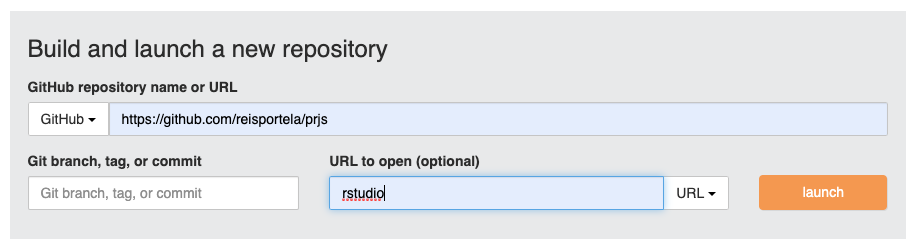
\includegraphics{figures/GESISNotebooks.png}

or a \textbf{Jupyter Lab}

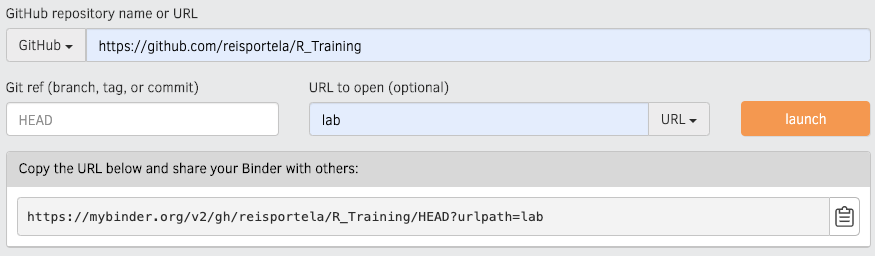
\includegraphics{figures/jupyter_lab.png}

\hypertarget{further-notes}{%
\section{11. Further notes}\label{further-notes}}

\hypertarget{jupyters-extensions}{%
\subsection{11.1 Jupyter's extensions}\label{jupyters-extensions}}

\emph{conda install -c conda-forge jupyter\_contrib\_nbextensions}

\emph{jupyter contrib nbextension install --user}

\hypertarget{kaggle-kernels}{%
\subsection{11.2 Kaggle Kernels}\label{kaggle-kernels}}

\href{https://towardsdatascience.com/introduction-to-kaggle-kernels-2ad754ebf77}{Kaggle}

\hypertarget{section}{%
\subsection{11.3}\label{section}}

\href{https://www.youtube.com/watch?v=rJsWJMBksK0}{How to Hide all the
code cells in Jupyter Notebook Python with single Click}

\hypertarget{pandas}{%
\subsection{11.4 Pandas}\label{pandas}}

\href{https://mybinder.org/v2/gh/jvns/pandas-cookbook/master}{Pandas
cookbook}

\hypertarget{r-and-dropbox}{%
\subsection{R and Dropbox}\label{r-and-dropbox}}

\href{https://github.com/karthik/rdrop2}{rdrop2}

\hypertarget{usefull-links}{%
\section{12. Usefull links}\label{usefull-links}}

\begin{quote}
\href{https://mybinder.org/}{Binder}

\href{https://codeocean.com/}{CODE OCEAN}

\href{https://notebooks.gesis.org/hub/home}{GESIS Notebooks}

\href{https://codeocean.com/}{Hypernet Labs}

\href{https://labs.cognitiveclass.ai/}{IBM Skills Network Lab}

\href{https://rstudio.cloud/}{RStudio Cloud}
\end{quote}

\begin{center}\rule{0.5\linewidth}{0.5pt}\end{center}

\hypertarget{how-to-prepare-a-singularity-script}{%
\section{How to prepare a Singularity
script}\label{how-to-prepare-a-singularity-script}}

\begin{enumerate}
\def\labelenumi{\arabic{enumi}.}
\item
  Download the script
  \href{https://github.com/reisportela/R_Training/tree/master/_containers/container_singularity.def}{container\_singularity.def}
\item
  Adapt the file to your project
\item
  Test the script at \href{https://cloud.sylabs.io/}{Sylabs} and build a
  Singularity image (e.g., my\_RStudio.sif)
\item
  Test the image
\end{enumerate}

\begin{itemize}
\item
  In your computer in case you have singularity installed
\item
  Use GitHub' CodeSpaces
\end{itemize}

\begin{enumerate}
\def\labelenumi{\arabic{enumi}.}
\setcounter{enumi}{5}
\tightlist
\item
  If you are running Linux do as follows:
\end{enumerate}

\begin{itemize}
\item
  Open a TERMINAL and type \texttt{singularity\ shell\ my\_RStudio.sif}
\item
  Once inside Singularity type \texttt{rstudio}
\item
  Now you can use your RStudio flavor within your computer and point to
  your data in \texttt{initial\_dataset}
\end{itemize}

\hypertarget{build-a-container-on-your-computer-using-singularity}{%
\section{Build a container on your computer using
singularity}\label{build-a-container-on-your-computer-using-singularity}}

\begin{enumerate}
\def\labelenumi{\arabic{enumi}.}
\item
  Install \texttt{singularity} from
  \url{https://sylabs.io/guides/3.0/user-guide/installation.html}
\item
  For Linux to install using package
\item
  For MacOs or Windows follow the instruction on on to install Vagrant
  and Vagrant Manager (you need to have Virtual box installed)
\item
  Difficulty: your computer must be able to run hardware accellarion
\item
  Specific notes on Vagrant
\end{enumerate}

\begin{quote}
Check details
\href{https://techtldr.com/how-to-copy-one-file-from-vagrant-virtual-machine-to-local-host/}{here}
\end{quote}

\begin{itemize}
\item
  open a Terminal and type \texttt{vagrant\ port}
\item
  you can copy files between your computer (\textbf{host}) and Vagrant
  (\textbf{guest}) using the following lines
\end{itemize}

\texttt{scp\ -P\ 2200\ vagrant@127.0.0.1:/vagrant/some-file.txt}

\texttt{scp\ -P\ 2222\ vagrant@127.0.0.1:/home/vagrant/containers/BPLIM\_Dashboard.sif\ .}

\begin{itemize}
\tightlist
\item
  in Vagrant you have \texttt{sudo} permissions
\end{itemize}

\begin{quote}
password:: \texttt{vagrant} login:: \texttt{vagrant}
\end{quote}

\hypertarget{build-and-use-the-vagrant-machine}{%
\subsection{Build and use the Vagrant
machine}\label{build-and-use-the-vagrant-machine}}

Open a Terminal and move to the folder of your choice

\begin{itemize}
\item
  Initialize a Project Directory:
  \texttt{vagrant\ init\ hashicorp/bionic64}
\item
  Install and Specify a Box:
  \texttt{vagrant\ box\ add\ hashicorp/bionic64}
\item
  Bring up a virtual machine: \texttt{vagrant\ up}
\item
  SSH into the machine: \texttt{vagrant\ ssh}
\item
  Build and image inside vagrant:
  \texttt{sudo\ singularity\ build\ BPLIM\_Dashboard.sif\ bplim\_Dashboard.def}
\end{itemize}

or
\texttt{sudo\ singularity\ build\ BPLIM\_Dashboard.sif\ bplim\_Dashboard.def}
in case you prefer a \texttt{sandbox}

\begin{itemize}
\item
  Test the image:
  \texttt{singularity\ shell\ -\/-writable\ build\ BPLIM\_Dashboard.sif}
\item
  Clean temporary files: \texttt{rm\ -rf\ /tmp/*}
\item
  Inside vagrant your host folder is mounted here \texttt{/vagrant}
\item
  Your \texttt{home} folder is located here \texttt{/home/vagrant}
\end{itemize}

\end{document}
